\documentclass{article}%
\usepackage[T1]{fontenc}%
\usepackage[utf8]{inputenc}%
\usepackage{lmodern}%
\usepackage{textcomp}%
\usepackage{lastpage}%
\usepackage[head=40pt,margin=0.5in,bottom=0.6in]{geometry}%
\usepackage{graphicx}%
%
\title{\textbf{Trabajadores del Metro protestaron en Chacao}}%
\author{El Nacional Web}%
\date{18/09/2018}%
%
\begin{document}%
\normalsize%
\maketitle%
\textbf{URL: }%
http://www.el{-}nacional.com/noticias/sociedad/trabajadores{-}del{-}metro{-}protestaron{-}chacao\_252182\newline%
%
\textbf{Periodico: }%
EN, %
ID: %
252182, %
Seccion: %
Sociedad\newline%
%
\textbf{Palabras Claves: }%
Metro de Caracas, Protestas, Sociedad\newline%
%
\textbf{Derecho: }%
2.3, %
Otros Derechos: %
, %
Sub Derechos: %
2.3.4\newline%
%
\textbf{EP: }%
SI\newline%
\newline%
%
\textbf{\textit{Los empleados de la compañía exigieron que se les haga el pago de convenciones colectivas}}%
\newline%
\newline%
%
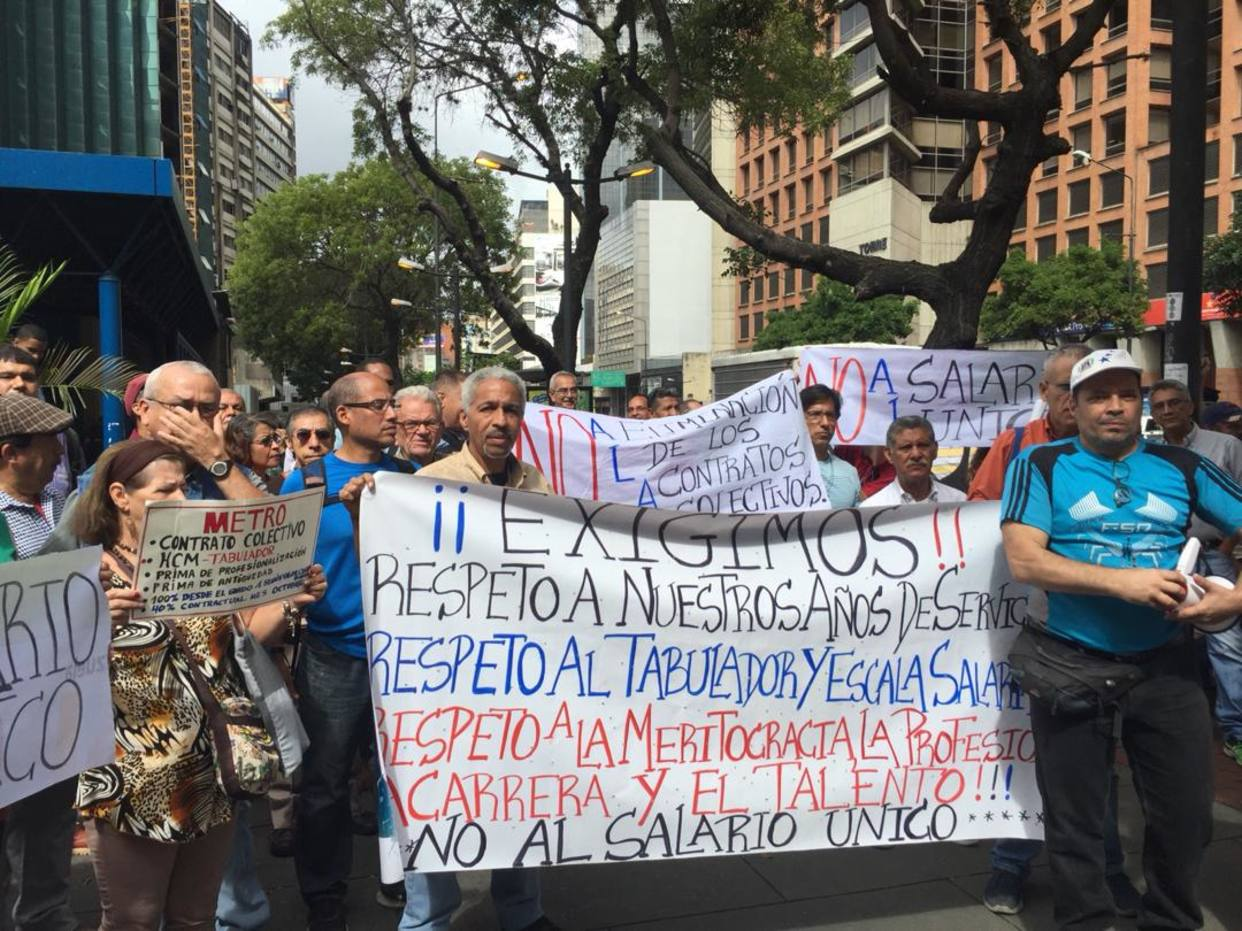
\includegraphics[width=300px]{109.jpg}%
\newline%
%
Empleados del Metro de Caracas protestaron~este martes a la altura de Chacao por contrataciones colectivas. Aseguraron~que no están dispuestos a perderlas porque tienen~años prestando servicio a la compañía.%
\newline%
%
Juan Ovalles, presidente de la Asociación de Jubilados y Pensionados del Metro de Caracas, informó que los trabajadores salieron a~la calle para exigirle al presidente del metro que respete las contrataciones colectivas.%
\newline%
%
A su vez, se refirió a la situación del Metro de Caracas y acotó que la institución está cerca de un paro técnico que, en cualquier momento, colapsará~las instalaciones.%
\newline%
%
“Seguridad, eficiencia y confort era el slogan que usaba en sus inicios la institución y actualmente ninguna de esas tres condiciones se cumplen. Para nadie es un secreto que tiene deficiencia en cuanto al rodamiento de trenes”, dijo Ovalles.%
\newline%
%
También se refirió al cobro del pasaje para usar el servicio y explicó que los torniquetes no están funcionando, por~lo que un miliciano “hace las veces de torniquete” para recoger los tickets de los usuarios%
\newline%
%
“El hombre tiene una bolsita para que la gente deposite el boleto ahí y quién sabe qué hacen luego con esos tickets porque aún son válidos para un pasaje”, acotó Ovalles.%
\newline%
%
\end{document}